%%%%%%%%%%%%%%%%%%%%%%%%%%%%%%%%%%%%%%%%%%%%%%%%%%%%%%%%%%%%%%%%%%%%%%%%%%%
% Copyright (c) 2010 committers of YAKINDU and others.
% All rights reserved. This program and the accompanying materials
% are made available under the terms of the Eclipse Public License v1.0
% which accompanies this distribution, and is available at
% http://www.eclipse.org/legal/epl-v10.html
%
% Contributors:
%     committers of YAKINDU - initial API and implementation
%%%%%%%%%%%%%%%%%%%%%%%%%%%%%%%%%%%%%%%%%%%%%%%%%%%%%%%%%%%%%%%%%%%%%%%%%%%

Now follows a quick introduction into the YAKINDU tools and the usage. For a
deeper understanding you can read the later chapters.
\section{The YAKINDU Perspective}
\begin{floatingfigure}[r]{0.3\textwidth}
  \centering
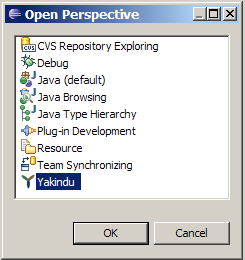
\includegraphics[width=0.3\textwidth]{./Pictures/yakinduPerspectiveSelection}
\caption{\label{fig:perspectiveSelection}Selecting the YAKINDU Perspective} 
\end{floatingfigure}
The YAKINDU tools comes with an easy perspective for quick starting and using it.
The perspective can be activate by clicking on \textbf{Window} $\rightarrow$
\textbf{Open Perspective} $\rightarrow$ \textbf{Other} and selecting the YAKINDU
perspective (Figure \ref{fig:perspectiveSelection}). After activation the screen
looks like figure \ref{fig:perspective}.

In the middle the main view on screen is the editor. It is still empty, but you
will use it most often. On the left is also a default eclipse view, the project
explorer. You will need it for the next step. The other views will be described
later, when they are needed.

\begin{figure}[ht]
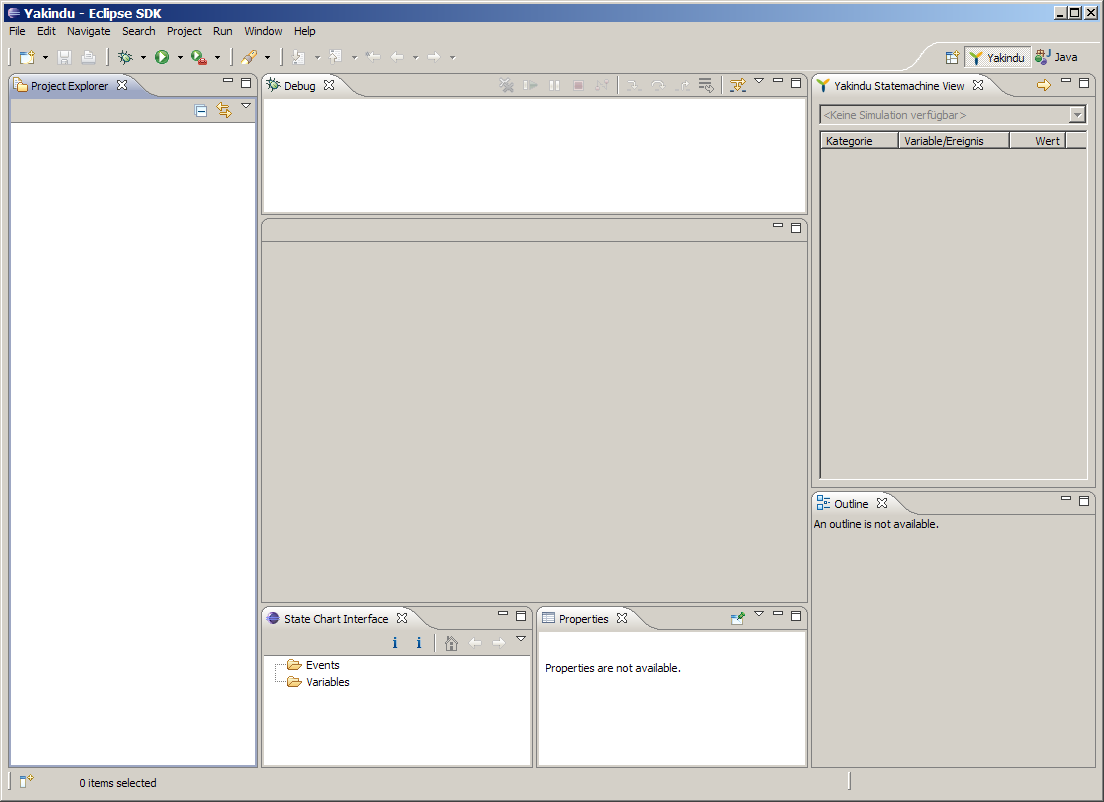
\includegraphics[width=0.5\textwidth]{./Pictures/perspective}
\caption{\label{fig:perspective}The YAKINDU Perspective} 
\end{figure}



\pagebreak
\section{Example Step by Step}

When YAKINDU is properly installed, we can start a small example project. This
example project gives an idea of how powerful the YAKINDU tool-chain is. It
contains a visual editor, a semantic and logic verification check, a simulator
unit and a number of code generators.

To present the visual editor, the check mechanism and the simulator of the
YAKINDU tool-chain, an example was chosen, that is simple enough to give an
impression of the usage but is not to far-fetched.

\subsection{Example State Machine}

The idea is to have a state machine, that represents a staircase lighting. This
staircase lighting is started with a key-press and stops after 30 seconds.

The state machine itself consists of two states: ,,Lights On'' and ,,Lights
Off''. The standard state within the state machine is ,,Lights Off'' and is
entered from start-up (the so called initial state). When an occupant enters the
staircase and presses the lighting button, a ,,keypress'' event is generated
which starts the transition to the ,,Lights On'' state.

On entering the state ,,Lights On'', the staircase lighting is turned on. When
the retention period has expired (after 30 seconds), the ,,Lights On'' state is
left with a transition to the state ,,Lights Off'' and the lighting is turned off
again.

\subsection{Creating a new Project}

When everything is set up, your Eclipse editor should look similar to this:

\begin{figure}[ht]
\centering
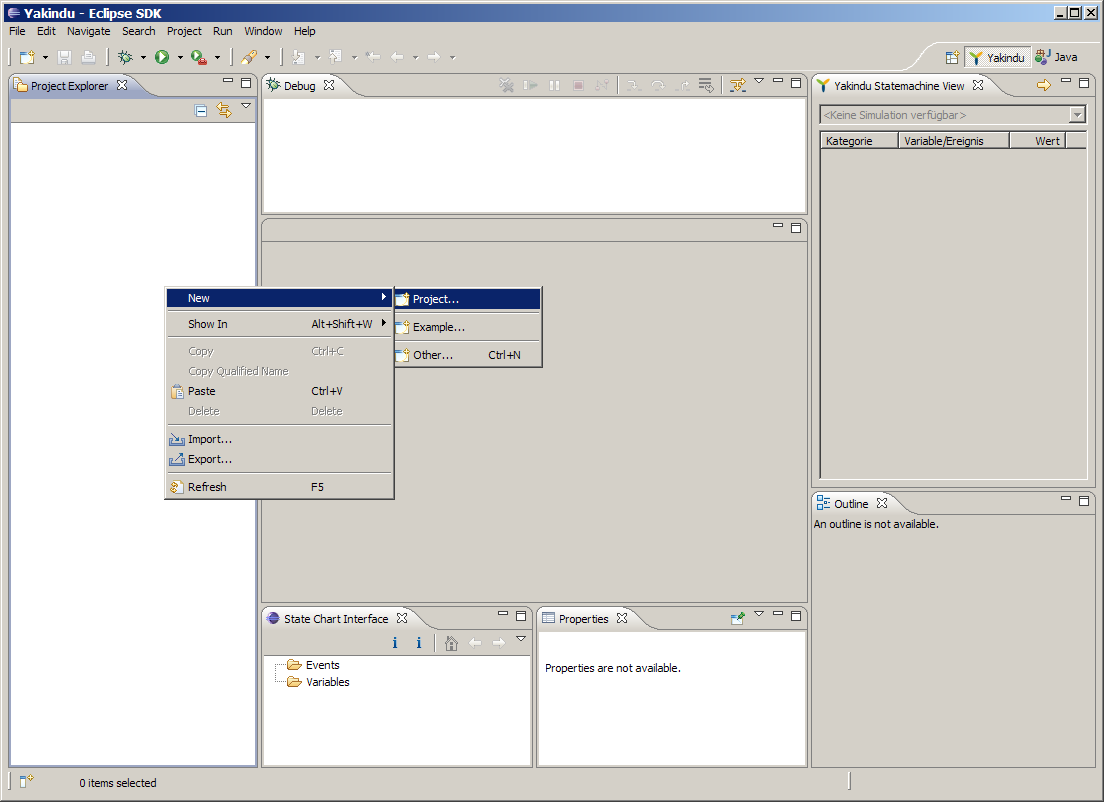
\includegraphics[width=0.8\textwidth]{./Pictures/NewProject}
\caption{\label{fig:NewProject}Creation of a new project} 
\end{figure}
\newpage
\begin{figure}[h!]
\centering
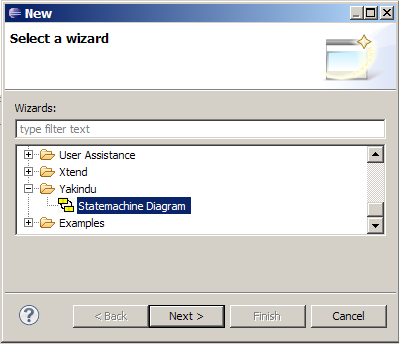
\includegraphics[width=0.5\textwidth]{./Pictures/Wizard}
\caption{\label{fig:wizard}Wizard to create a new State Machine}
\end{figure}

To start a new project, open the menu (\textbf{File$\rightarrow$ New$\rightarrow$
Project}) and create a new Java Project. In our example, the project is called
,,\textit{Example}''.  However, this procedure only creates a default Java
project. For simplicity you should deny the question for changing to Java
perspective, because we won't use anything from Java. \newpage
\begin{floatingfigure}[r]{0.3\textwidth}
\centering
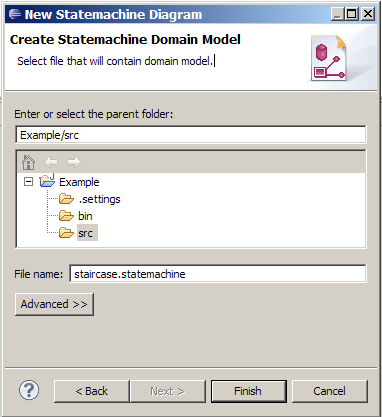
\includegraphics[width=0.3\textwidth]{./Pictures/Wizard2}
\caption{\label{fig:wizard2}Wizard to create a new state machine domain model}
\end{floatingfigure}
To create a \textbf{state machine model} to this environment, right-click the
\textbf{src} directory icon and open the select wizard at
\textbf{New$\rightarrow$ Other}. Here you have to select \textbf{state machine
Diagram} from the \textbf{YAKINDU} folder as shown on figure \ref{fig:wizard}.

Figure \ref{fig:wizard2} displays the \textit{New Statemachine Diagram} window,
in which the name of the state machine model is set. In our example, the name is
changed from \textbf{default.statemachine} to staircase.statemachine.

The wizard has then created two sources: the \textbf{staircase.state\-machine}
and the \textbf{staircase. state\-machine\_\-diagram}. The state machine itself
is represented as an XML-file in \textbf{staircase. state\-machine} and the
visual representation of the state machine can be found in the
\textbf{staircase.state\-machine\_\-diagram} file.


Now you should have a new visual editors view to create a state machine as shown
in figure \ref{fig:YEditor}. Here you have all elements to create a state machine
from bottom up in the elements menu. The elements that are important for our
small project are 
\includegraphics[height=12pt]{./Pictures/Region},

\includegraphics[height=12pt]{./Pictures/State},

\includegraphics[height=12pt]{./Pictures/Transition} and

\includegraphics[height=12pt]{./Pictures/InitialState}.

\begin{figure}[ht]
\center
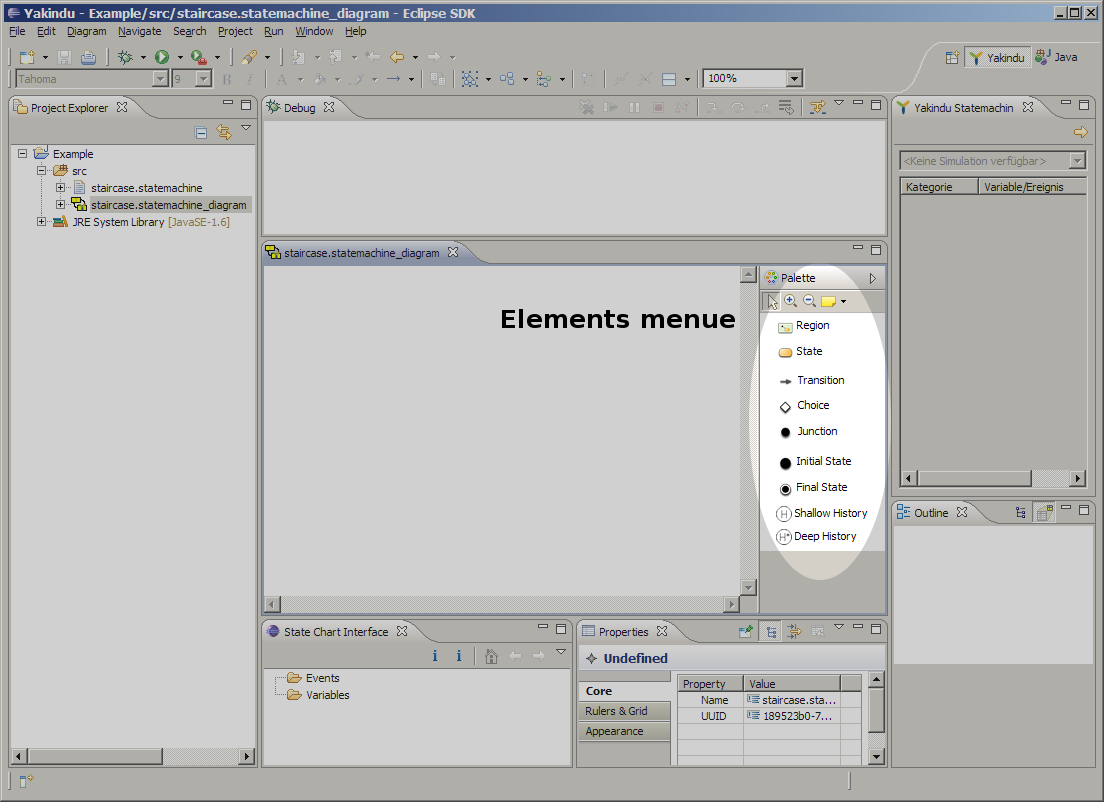
\includegraphics[width=\textwidth]{./Pictures/YakinduEditor_1}
\caption{\label{fig:YEditor}YAKINDU State Machine editor}
\end{figure}
 
\subsection{Defining a State Machine}

%Creating a state machine is quite easy:

To start with the visual editor you firstly need a region, in which the states of
the state machine reside. Therefore you need to click the

\includegraphics[height=12pt]{./Pictures/Region} icon and draw a region on the
empty plain. When you have placed the last corner of the region and you release
the mouse button, a new region in light green appears. At the properties area,
the priority of this region is highlighted and should be set to a value. As we do
not have any concurrent regions in this example, the priority is not important
and could be set to any valid integer value (10 in our example). If you use more
than one region, the priority specifies the processing order in which the states
actions and the states transitions are processed.

% ToDo (for further information please refer to section \ref{sec:Regions}).

To set the priority of the region afterwards, you can open the properties view.
If you cannot find it in your eclipse perspective, you can open it by clicking
\textbf{Window$\rightarrow$ Show View$\rightarrow$ Others} and in that menu:
\textbf{General$\rightarrow$ Properties}.

Now as you have created a region, you need a starting point of your state
machine. This starting point is called \textbf{initial state} and can also be
found as an icon (
\includegraphics[height=12pt]{./Pictures/InitialState}) in the
elements menu. As explained at the beginning of this chapter, the two states
\textbf{LightOn} and \textbf{LightOff} should be installed within the state
machine region.

To create a state, you have to select the
(
\includegraphics[height=12pt]{./Pictures/State}) element and then open the area
within the region plain. When the state outline is created, the first line within
the properties area is highlighted and needs to be filled by the name of this
state (e.g. LightOff). The name of a state has to be unique within a region.

\begin{figure}[ht] \center
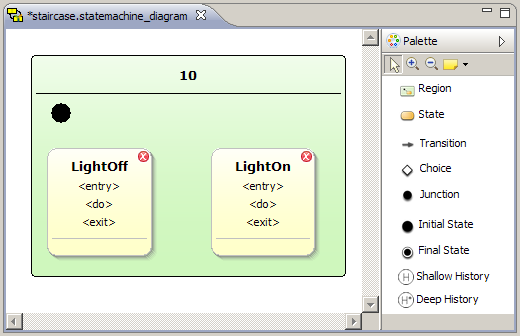
\includegraphics[width=0.7\textwidth]{./Pictures/StateCreation_1}
\caption{\label{fig:StateCreation}Creation of the \textbf{Initial}, 
\textbf{LightOff} and \textbf{LightOn} state}
\end{figure}
% \clearpage

After the creation and naming of the states, the actions ($<entry>$, $<do>$,
$<exit>$) should be created. In our case, the only action that should be
performed is switching the light on or off. The status of the light is
represented by a variable that could hold one of the two values 1 or 0. This
variable needs to be created in the \textbf{State Chart Interface}. Within this
view, you can right-click on \textbf{Variables}, where you get a new window to
specify the variable that should be created (refer figure
\ref{fig:CreateVariable}). Here you add the variable name (\textit{Light}), the
port, the IO-type and the data type. In our example all other information except
for the variable name do not have to be changed.

\begin{floatingfigure}[r]{0.4\textwidth}
\includegraphics[width=0.4\textwidth]{./Pictures/CreateVariable}
\caption{\label{fig:CreateVariable}Creating a variable in the \textit{State Chart Interface}}
\end{floatingfigure}

%\begin{figure}[ht]
%\center
%\includegraphics[width=0.3\textwidth]{CreateVariable}
% \caption{\label{fig:CreateVariable}Creating a variable in the \textit{Data
% Element Explorer}} \end{figure}

Then you add the action \texttt{Light=0;} into the $<entry>$ line within the
states properties area (either within the Diagram or within the
\textbf{Properties} view). This definition creates a new action, that is
performed whenever the state \textbf{Light\-Off} is entered. So when the
unconditioned state transition from the \textbf{initial state} to the
\textbf{LightOff} state is performed, the internal variable \textit{Light} is set
to zero. The same takes place, when the state \textit{LightOff} is entered
through a transition from any other state.

The state \textbf{LightOn} is created in the same way, except that the action is
set to \texttt{Light=1;}.

To create a transition between the \textbf{Initial State} and the
\textbf{LightOff} state, you choose the

\includegraphics[height=12pt]{./Pictures/Transition} element and connect the
\textbf{Initial State} and the \textbf{LightOff} state. Every transition claims
an \textbf{expression}, when this transition should be executed.

An expression can consist of one or more \textit{triggers}, \textit{guard
operations} and \textit{actions}, which can also be mixed. Additionally a
transition must have a priority, to define the order, in which the expressions of
different, concurrent transitions are processed.
% ToDo To learn more about transition expressions, please read section
% \ref{sec:Transitions}.

In our example, the transition between the \textbf{Initial state} and the
\textbf{LightOff} state do not need any expression, as this transition has no
condition. When the expression area of a transition is left blank, the expression
is represented by an asterisk (*).

The transition between \textbf{LightOff} and \textbf{LightOn} is performed, if
the trigger \textit{keypress} was received. Therefore a new event has to be
implemented in the \textit{State Chart Interface} (refer also to figure
\ref{fig:CreateVariable}). Here you add an event that can be used as a trigger
within a transition expression. Implementing a trigger with a transition needs
only the trigger name as the expression string (\textit{keypress}).

To specify the transition from \textbf{LightOn} to \textbf{LightOff} after 30
seconds, you use the keyword $after(<duration>s)$ within the transition
expression string. The \textit{after()} expression switches to the target state
when the specified time has been expired.

So in the end your state machine looks like in figure
\ref{fig:statemachineFinish}.

\begin{figure}[ht]
\center
\includegraphics[width=0.7\textwidth]{./Pictures/statemachineFinish_1}
\caption{\label{fig:statemachineFinish}Complete State Machine (State Machine Diagram Editor)}
\end{figure}

\newpage
\subsection{Checking the State Machine}
The state chart is very common and it is possible to model things, which doesn't
make sense for your target platform or you want to have some special naming
conventions. We will check now, that every name of a state is at least eight
character long. But first we have to prepare our Project for code completion
within checks. Later on we can add a new check file and enter the checks.

\subsection{Project type and dependencies}
For this steps it is neccessary, that the model is inside an Java project. If
it's not yet, you can create a new project beside the first, copy the model and
change the target directories (see chapters \ref{sec:CCodeGenerator} and
\ref{sec:JavaCodeGenerator})  for generated files, so they point to the first.

\begin{figure}[ht]
\center
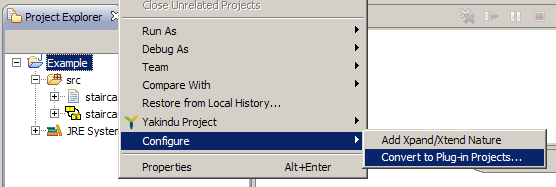
\includegraphics[width=0.7\textwidth]{./Pictures/switch_to_pde_project}
\caption{\label{fig:switchToPdeProject}Add plugin development nature to your java project}
\end{figure}
We will add the plugin development nature from eclipse to the project by
selecting the project, click with the right button and select \textbf{Configure}
$\rightarrow$ \textbf{Convert Projects to Plugin Projects\dots} (Picture
\ref{fig:switchToPdeProject}). Your project is already selected in the next
window and you can press Finish to complete. As a result some new files are
created in your project. We only need the \textbf{MANIFEST.MF} inside the folder
\textbf{META-INF}. Open this file by double-click and add some dependencies (See
picture \ref{fig:manifest}). This is done by clicking on \textbf{Add} and
selecting some plugins. If you design for codegeneration the plugin
\textit{com.yakindu.statechart.codegenerator.java} or
\textit{com.yakindu\dots{}c} are the one of your choice. For platform independent
modeling you can select \textit{com.yakindu.statechart.model.expressions}.
\begin{figure}[ht] \center
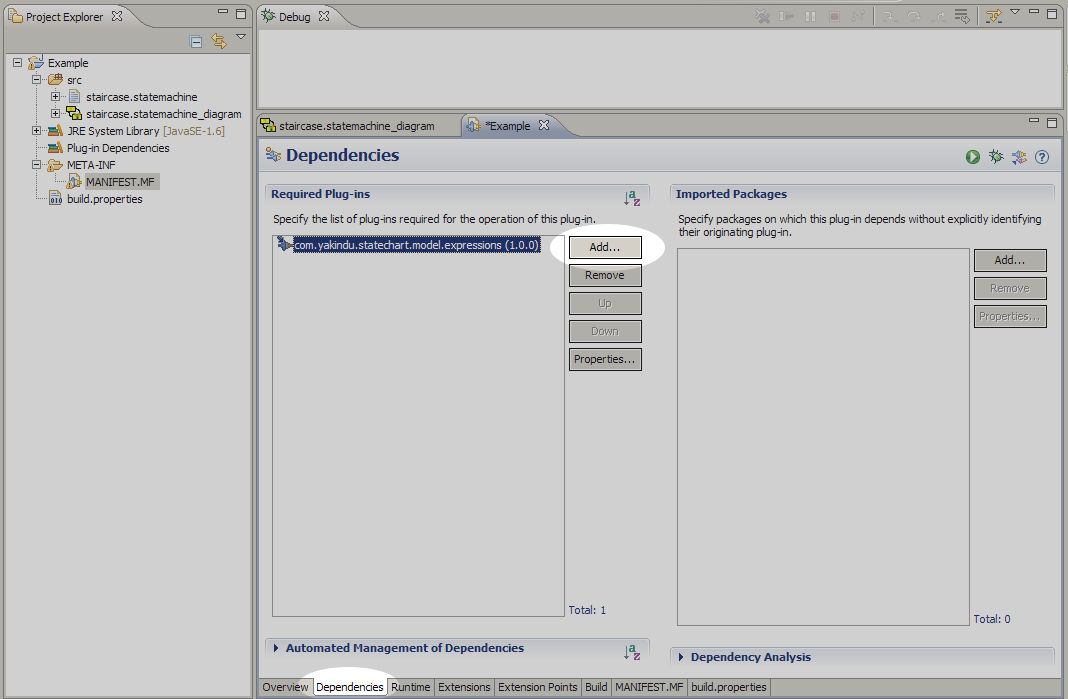
\includegraphics[width=0.7\textwidth]{./Pictures/manifest}
\caption{\label{fig:manifest}Add dependencies to your project}
\end{figure}

Now the file can be saved and closed. It will not be neccessary to edit this file
later, except you decide to use an additional codegenerator.

\subsection{Create check files}
All user defined check files reside in a folder names checks. Within this folder
all \textbf{.chk}-files are evaluated and considered for checking. The format of
check files is described in the reference of eclipse modeling project and the old
openArchitectureWare-project\footnote{http://oaw.itemis.de/openarchitectureware/662/ressourcen}.

Create a new folder in the root of your project by right-click on
\textbf{Examples}  and selecting \textbf{New}$\rightarrow$\textbf{Folder}. The
folder must be named \textit{checks} and the other options can be ignored. Simply
finish and create your check files inside this folder.

Check files are created by selecting the folder ''checks'' and choosing in the
drop-down-menu the entry \textbf{New}$\rightarrow$\textbf{Other}. In the next
window the entry \textbf{Check file} is found inside the category
\textbf{Xtend}(see Figure \ref{fig:newCheckFile}.

\begin{figure}[ht] \center
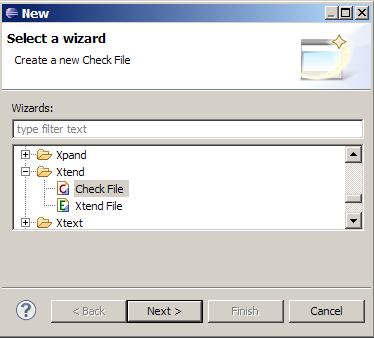
\includegraphics[width=0.7\textwidth]{./Pictures/newoAWCheckFile}
\caption{\label{fig:newCheckFile}Add a new check file to your project}
\end{figure}

\subsection{Editing check files}
The syntax of check files is described in the oAW-Reference, but the short
introduction here is enough for the first experience. If you try the code
completion (\texttt{Strg+space}) the first time in the editor, you are asked to
add the Xtend nature to your project (See figure \ref{fig:addOAWNature}). Answer
with yes, to get code completion. \begin{figure}[ht] \center
\includegraphics[width=0.7\textwidth]{./Pictures/addoAWNature}
\caption{\label{fig:addOAWNature}Add the Xtend nature to your project for code completion}
\end{figure}

Every check file starts with an \texttt{import} of the required and used models.
For the statemachine it is sufficient to add the model \texttt{statemachine}.
After this we want to add a check for a state. This is done by defining a
\texttt{context} for the model element \texttt{State} and the severity of
\texttt{WARNING} or \texttt{ERROR}. Because short names are not nice and we
spelling names we define an error with the error message ''State names must have
at least 8 characters''. After a colon the boolean expression folows. The
expression defines the default, not the error. In our case names are longer or
equals to eight characters. In figure \ref{fig:nameLengthCheck} the result of
''state.chk'' is printed.

\begin{figure}[ht] \center
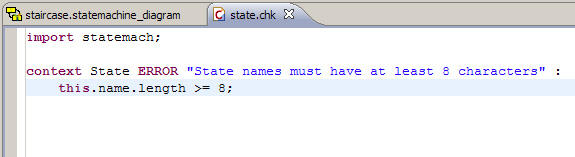
\includegraphics[width=0.7\textwidth]{./Pictures/nameLengthCheck}
\caption{\label{fig:nameLengthCheck}An example check file for names longer 
than eigth characters}
\end{figure}

After saving the file and opening the statechart again, the statechart is
validated after some seconds. As a result you can see a red cross in the upper
right corner of state LightOn. That's because we added a check, that state names
must have at least eight characters and LightOn needs only seven characters. If
you put the mouse above the red cross and wait some seconds, the error message is
shown in a small box.

\subsection{Simulating a State Machine}
\label{sec:simulatingStateMachine}
When the state machine diagram is completed, you can start a simulation session,
to check, whether your new state machine is working correctly.

To start a simulation you have to create a new \textit{run} configuration, as
shown in figure \ref{fig:SimulationStart}. Choose the entry \textbf{Run
Configuration ...} to open the configuration dialog.

\begin{figure}[ht] \center
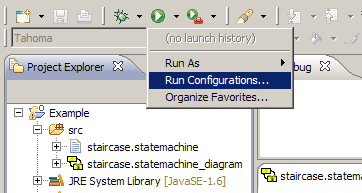
\includegraphics[width=0.4\textwidth]{./Pictures/startSimulation_1}
\caption{\label{fig:SimulationStart}Starting the Simulation creation dialog}
\end{figure}

In this dialog you add a new \textbf{YAKINDU Simulation} called \textit{Example}
by clicking the 'New' button in the upper left corner. Then the configuration
dialog is presented. After choose your \textit{Example} project and the staircase
state machine as your model file the dialog looks like figure
\ref{fig:SimulationCreation}. As your simulation engine, please choose
\textit{YAKINDU Statechart Simulator}.

\begin{figure}[ht]
\center 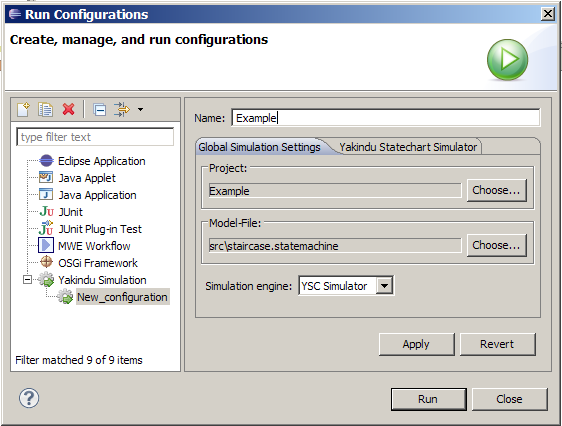
\includegraphics[width=0.7\textwidth]{./Pictures/SimulationCreation}
\caption{\label{fig:SimulationCreation}Dialog to create a new simulation environment}
\end{figure}

When you click the \textbf{Run} button in the lower right corner, you start the
simulation. To rerun the simulation later, you find an entry \textit{Example} in
your \textbf{Run} configuration.

\begin{figure}[ht] \center
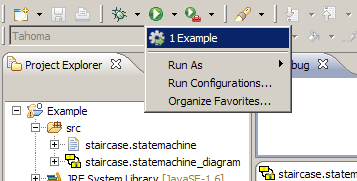
\includegraphics[width=0.4\textwidth]{./Pictures/runLater_1}
\caption{\label{fig:runLater}Restart a simulation in the menu}
\end{figure}

On Simulation start-up make sure, that the debug view is open (refer figure
\ref{fig:runningSim_1}). In this view, the simulation process can be started,
stopped and paused. Additionally the simulation can be used in single step modus.
To activate the single step modus, the simulation must be in the pause position.
When a single step should be performed, the single step button can be pressed.
The advantage in this modus is, that you can set the input parameter according to
your simulation scenario and perform the next step, when you are done with that.
To be able to change the events and variables, you must have started the
simulation explicit by a click to the run button in the debug view, or by
clicking on the single step button.

To be able to interact with the simulation by the input values, open the
\textbf{YAKINDU Statemachine View}. This view can be found in the main menu under
\textbf{Window}$\rightarrow$ \textbf{Show View}$\rightarrow$ \textbf{Other...}.
In the appearing menu choose \textbf{YAKINDU Statemachine}.

\begin{figure}[ht] \center
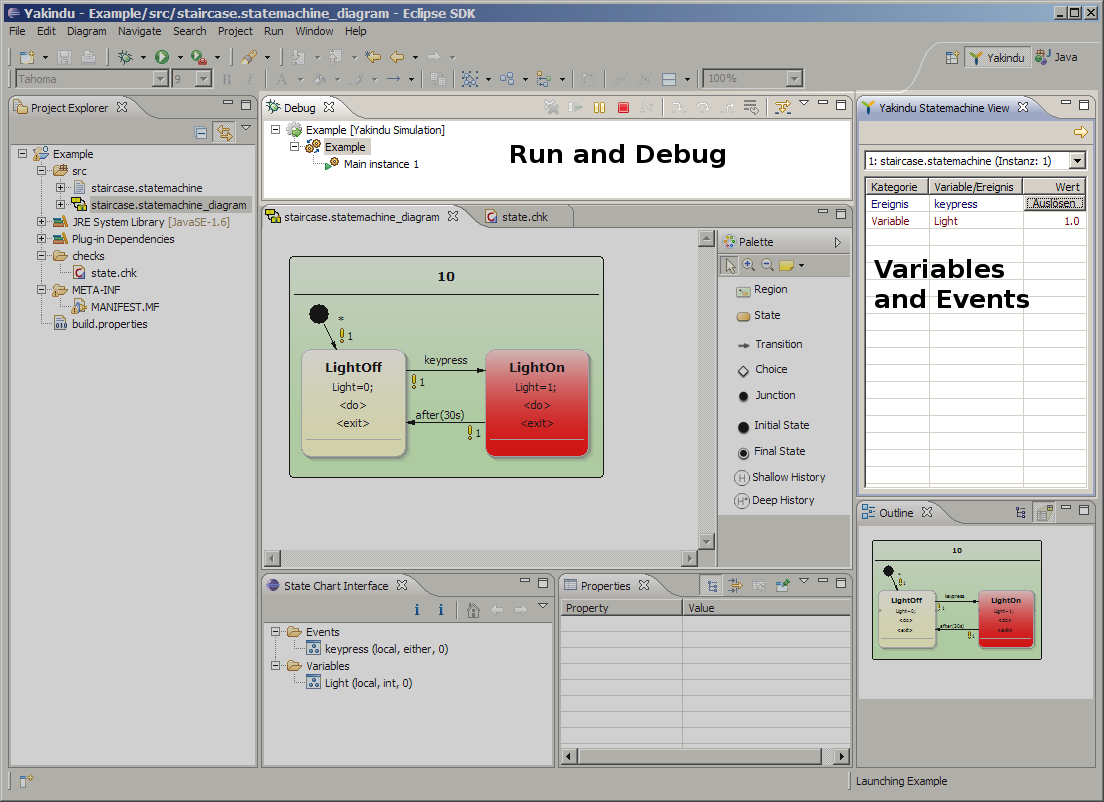
\includegraphics[width=0.7\textwidth]{./Pictures/runningSim_1_1}
\caption{\label{fig:runningSim_1}Running a simulation}
\end{figure}
 
% \begin{floatingfigure}[r]{0.3\textwidth}
% 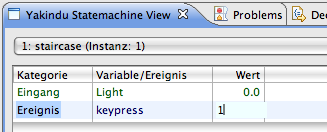
\includegraphics[width=0.3\textwidth]{./Pictures/runningSim_2}
% \caption{\label{fig:runningSim_2}Change trigger value during simulation}
% \end{floatingfigure}

In our example project, the state machine starts with a transition from the
initial state to the \textit{LightOff} state. This state transition is visualized
by a red arrow. During a simulation an active state is highlighted in red.

\begin{figure}[ht] \center
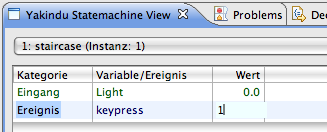
\includegraphics[width=0.4\textwidth]{./Pictures/runningSim_2}
\caption{\label{fig:runningSim_2}Change trigger value during simulation}
\end{figure}

After the active state has changed into \textit{LightOff}, this state can only be
left by a transition to \textit{LightOn}. The condition expression is set to the
trigger \textit{keypress}. This trigger can be created in the YAKINDU
Statemachine View during simulation time.  To simulate a keypress, just click the
''fire'' button near the \textit{keypress} event in Statemachine view. In this
case, the value changes and the transition is followed. After the transition has
been performed, the trigger for the transition is reset.

\begin{figure}[ht] \center
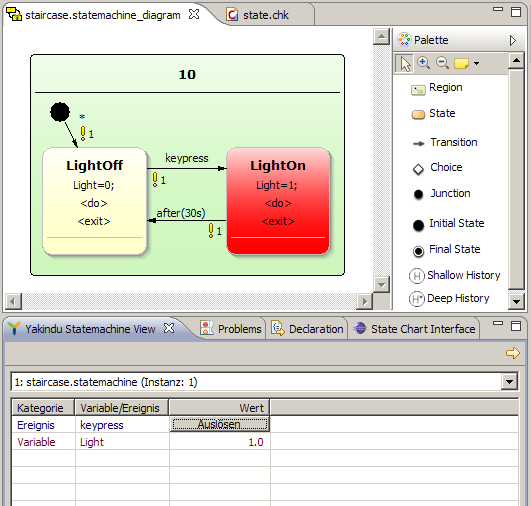
\includegraphics[width=0.7\textwidth]{./Pictures/runningSim_3}
\caption{\label{fig:runningSim_3}Trigger \textit{keypress} was activated and
the state \textit{LightOn} has been reached}
\end{figure}

The same procedure is valid to set a value of a variable. The difference between
a variable and a trigger is that a trigger value is reset to zero as soon as the
trigger has taken effect, e.g. a transition was successful. A variable value is
only changed when it is actively changed by the user or an action e.g. in
$<entry>$ $<do>$ or $<exit>$.


\pagebreak
\section{Using Example Projects}
\label{sec:exampleProjects} 

Some example projects are included in the YAKINDU release. They can be installed
by creating the \textbf{Statemachine example project}. This is done by selecting
\textbf{File} $\rightarrow$ \textbf{New} $\rightarrow$ \textbf{Statemachine
example project}. This Wizard (see Figure \ref{fig:exampleWizard}) creates after
all three new projects in your workspace, called ''Safe'', ''StaircaseLighting''
and ''TrafficLight''. You can read a short description of them, if you select
one. After you click finish the new projects are listed in your project explorer.

\begin{figure}[ht] \center
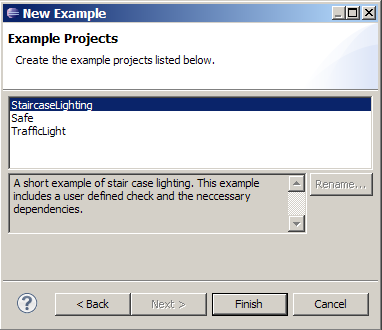
\includegraphics[width=0.6\textwidth]{./Pictures/examplesWizard}
\caption{\label{fig:exampleWizard}The state machine examples} 
\end{figure}

Taking a deeper look at the files inside the examples (Figure
\ref{fig:easyExamples}), the two projects Safe and StaircaseLighting contain only
two files. The \textit{.statemachine} file contains the model of your state
machine, and the \textit{.statemachine\underline{ }diagram} file is for
modelling. Both files are necessary to simulate and visualize the simulation. If
no visualization is needed, the model themself is enough. How to simulate is
described in section \ref{sec:simulatingStateMachine}.

The files inside the third project, the TrafficLight model, includes also model
files inside the model directory, but also an workflow under workflow and an
complex simulation environment for practical usage with a microcontroller. This
set up and handling is described in the next section \ref{sec:CCodeGenerator}

\begin{figure}[htbp] \center
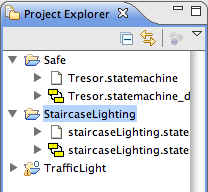
\includegraphics[width=0.3\textwidth]{./Pictures/easyExamples}
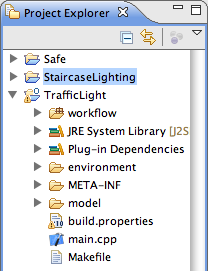
\includegraphics[width=0.3\textwidth]{./Pictures/complexExample}
\caption{\label{fig:easyExamples}Example projects and files inside} 
\end{figure}

Now we will start with a short hands-on example to demonstrate how development is
done and what especially the elements and views are for. This step is orthogonal
to-the-ready to use examples in this section.

\clearpage
